\chapter{Introduction}
	\section{Chapter Overview}
		To open the thesis, this chapter gives a brief background of why the project is being pursued in the law domain. It continues by explaining the project's aims with regards to the given background and then finishes with how the aims intended to add value to the law domain once they had been met. 
	\section{Project Context}
		Intellectual Property law is a term typically used to describe the areas of law which establish property protection over intangibles such as ideas, signs and information. This protection is in order to make the advancement of ideas profitable which therefore incentivises this act\cite{ip_edu_bently}.
			
		There is, therefore, a balance to be struck between limited exclusive rights and benefits to the public. While limiting exclusive rights may facilitate progress, benefiting the public, the overprotection of the exclusive property may restrict their access\cite{handbook_ip_hr_geiger}. One example of this is the expansion of copyright terms such as the controversial Copyright Term Extension Act of 1998 which was heavily lobbied for by Disney just years before Mickey Mouse's copyright ran out\cite{mickey_mouse_grzelak}. The trend in extension of copyright terms, illustrated by Figure \ref{fig:ext_us_cop}, illustrates the appearance that the balance is tipping towards exclusivity rights. 

		\begin{figure}[h]
    		\centering
    		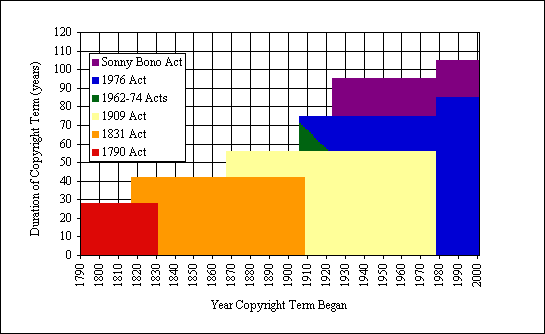
\includegraphics[width=0.5\linewidth]{resources/images/extention_of_us_copyright.png}
    		\caption{Expansion of U.S. copyright term lengths\cite{copyright_term_length_graph_bell}.}
    		\label{fig:ext_us_cop}
		\end{figure}
			
		This implementation of intellectual property law brings in the question of human rights of access to culture, education and other social and economic rights, but traditionally this has not been included in discussion of intellectual property law. However, recently scholarship and legislation has progrssively begun to incorporate each other's linguistics\cite{mapping_ip_hr_helfer}.
			
		Dr. Megan Rae Blakely of Lancaster University is looking for assistance in analysing journals and legal instruments for overlap in languages. As well as the human rights and intellectual property, Dr. Blakely hypothesised that it may be interesting to see how the language in these fields benefit the user and the creator of intellectual property\cite{bileta_proposal_blakely}. In this analysis, I will map the dynamics of this change in legal and social perspective, to make evident moments of significant shifts in language. 
			
		Previously, analysis of the intersection between human rights and intellectual property law, such as Helfer's\cite{hr_ip_conflict_coexistence_helfer}, has been limited to more manual case-by-case methods. Supplying a more systematic method using natural language processing that can cope with large amounts of data would give concrete evidence of the relationship between human rights and intellectual proeprty. 
	\section{Ground Truths}
		Dr. Blakely supplied a set of ground truths that she wished to analyse the language of. This consisted of the following:
		\begin{itemize}
			\item Four journals, shown in Table \ref{tab:journal-list}: two that are on the topic of human rights and two that are on the topic of intellectual property;
			\item Four international treaties, shown in Table \ref{tab:treaty-list}: two that are on the topic of human rights and two that are on the topic of intellectual property;
			\item Four lists of words, shown in Table \ref{tab:keyword-list}: one that Dr. Blakely expects to see in documents about human rights, one that Dr. Blakely expects to see in documents about intellectual property, one that Dr. Blakely thinks indicates that a segment indicates benefits to the user and one that Dr. Blakely thinks indicates that a segment indicates benefits to the creator.
		\end{itemize} 
	\section{Requirements}
		In the early stages of the project, I worked with Dr. Blakely to establish a set of requirements for the project. These requirements can be split into three categories: natural language processing, visualisation, and usability.  

		Each of the following subsections discusses the requirements of a different category. Each subsection starts by specifying the deliverable elements for the category, followed by high-level criteria of how they will be evaluated. All goals needed to be completed by 16th April 2019, when Dr. Blakely presents to the British and Irish Law Education and Technology Association (BILETA) Conference. 
		\subsection{Natural Language Processing}
			The natural language processing in the project will take the form of two models. Each model will take the same corpus of training PDF documents as input but will classify different characteristics of the corpus.
			
			\begin{itemize}
				\item The first model will use topic classification to identify whether a document is related more to human rights or intellectual property;
				\item The second model will use sentiment analysis to identify whether the document indicates that the current legal climate more strongly benefits the user of intellectual property of the creator of it.
			\end{itemize}
			
			It is notable that Dr. Blakely expressed that the former is the more important model in terms of the project's success as there is more scholarly work done on this relationship. The latter models' relationship is less widely covered and was requested by Dr. Blakely as a personal preference. 

			These models will be successful if they meet the following criteria: 
			\begin{itemize}
				\item The model accurately represents a large proportion of the documents in the corpus with regards to its classification characteristics; 
				\item The model deduces any trends in the corpus with regards to its classification characteristics, if those trends exist; 
			\end{itemize}
			
			The model must only consider the language of the content of the article. 
		\subsection{Visualisation}
			The previously mentioned models will then have to be visualised. Dr. Blakely stated her belief that a modification of Eboch's tone graph\cite{tone_graph_eboch} shown in Figure \ref{fig:eboch_adapt} would be a suitable visualisation for the models. This would involve an x-axis representing time, a y-axis representing human rights-intellectual property and a z-axis representing user-creator. 
			
			\begin{figure}[h]
    			\centering
    			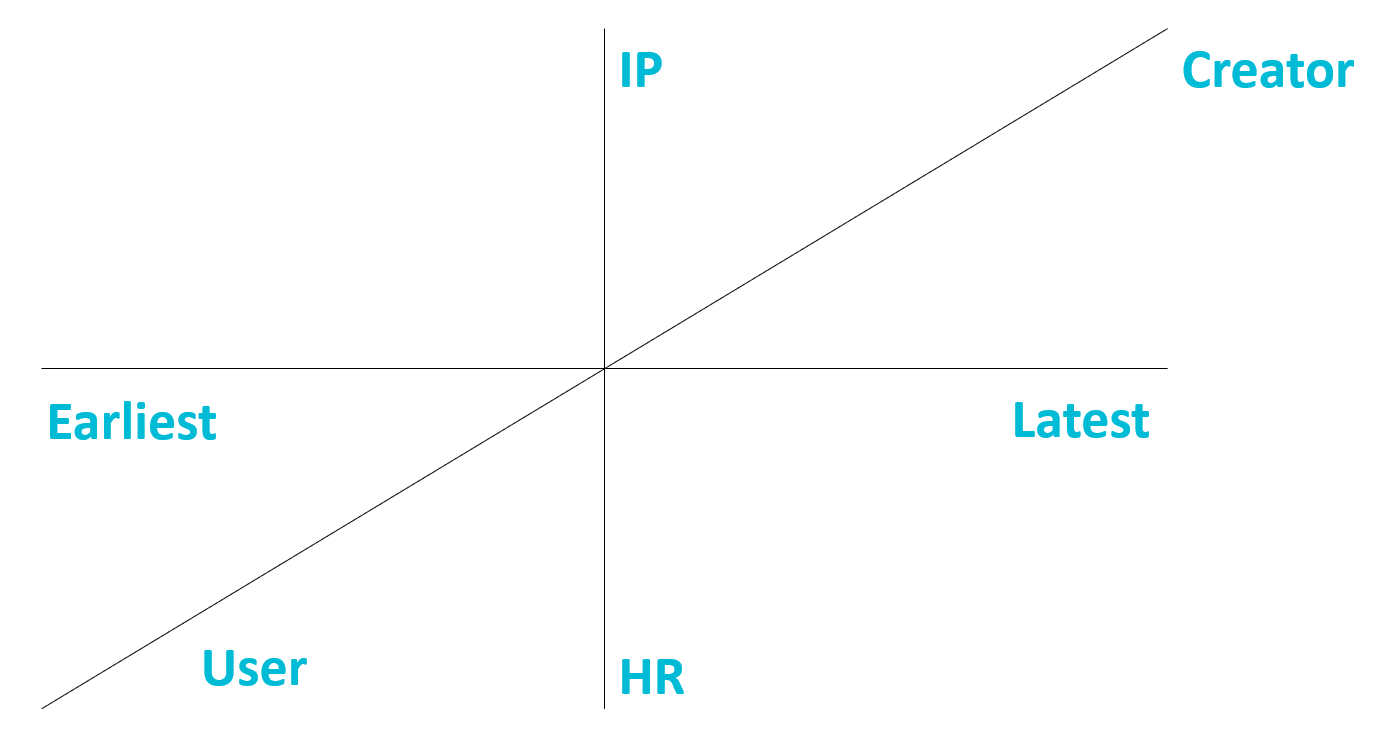
\includegraphics[width=0.5\linewidth]{resources/images/eboch_adapt.png}
    			\caption{An adaptation of Eboch's tone graph for this domain.}
    			\label{fig:eboch_adapt}
			\end{figure}
			
			The visualisation will be successful if it meets the following criteria:
			\begin{itemize}
				\item The visualisation and its axes' meanings are self-explanatory; 
    			\item It is clear where a point lies on the visualisation's axes; 
    			\item The visualisation has all the possible information that Dr. Blakely requires, on it; 
    			\item The visualisation clearly indicates any trends deduced by the models; 
    			\item The visualisation is aesthetically pleasing. 
			\end{itemize}
			
		\subsection{Usability}
			There will be two key types of stakeholders in this project. Both their circumstances will have to be considered in order to deliver a suitable final product. 

			The first type of stakeholder are the users of the project's end product. This will primarily be Dr. Blakely but is likely to extend to other law academics. It is important to note that these will likely be people with standard information technology skills and no computer science skills. Therefore, the end product will need to be in the form of a tool that is accessible to people of this calibre.  

			The tool must have the following features: 
			\begin{itemize}
				\item Allow for input of new documents;
				\item Display visualisations based on models with given documents as input;
				\item Display information about success of model.
			\end{itemize}

			The tool will be successful if it meets the following criteria: 
			\begin{itemize}
				\item The tool does not require any prior Computer Science knowledge to setup or use;
				\item The tool has a graphical user interface which is intuitive; 
			\end{itemize}
			
			The second type of stakeholder is the future developers furthering Dr. Blakely's research. These developers will be experts in natural language processing and computer science and so will be able to both use and change the tool to their liking. However, changes to the tool will only be easily changeable if the codebase for it is well written. 

			The codebase will be successful if it meets the following criteria:
			\begin{itemize}
				\item It is easy to understand the purpose of each section of code;
				\item It is easy to expand upon and adapt the overall codebase.
			\end{itemize}

		\section{Added Value}
			This project is original in its application of natural language processing methods to find the relationship between intellectual property and human rights language. None of the individual computing methods used were original, but the added value appears through the iterative process which found the most appropriate visualisation of results for the domain. The outcome of the project will help add value to its domain by illustrating how historical changes in technology have impacted the tone of intellectual property law. Blakely points out that this, in turn, will allow legal professionals to consider how future technological changes will impact their work and adapt accordingly.